\documentclass{extbook}
\usepackage[utf8]{inputenc}

\usepackage{mathtools}
\usepackage{listings, xcolor}
\usepackage{color}
\usepackage{geometry}
\usepackage{graphicx}
\usepackage{proof}
\usepackage{syntax}
\usepackage{hyperref}
\usepackage{tikz-qtree}

\DeclareUnicodeCharacter{03BB}{$\lambda$}
\DeclareUnicodeCharacter{03C4}{$\tau$}
\DeclareUnicodeCharacter{03B1}{$\alpha$}
\DeclareUnicodeCharacter{27F6}{$\rightarrow$}
\DeclareUnicodeCharacter{0393}{$\Gamma$}
\DeclareUnicodeCharacter{2205}{$\emptyset$}
\DeclareUnicodeCharacter{0394}{$\Delta$}


\newgeometry{
left=   1 in,
bottom= 1.5 in,
right=  1 in,
top=    1 in
}

\definecolor{bluekeywords}{rgb}{0.13,0.13,1}
\definecolor{greencomments}{rgb}{0,0.5,0}
\definecolor{turqusnumbers}{rgb}{0.17,0.57,0.69}
\definecolor{redstrings}{rgb}{0.5,0,0}

\lstdefinelanguage{FSharp}
		{morekeywords={let, new, match, with, rec, open, module, namespace, type, of, member, and, for, in, do, begin, end, fun, function, try, mutable, if, then, else,type},
    keywordstyle=\color{bluekeywords},
    sensitive=false,
    morecomment=[l][\color{greencomments}]{///},
    morecomment=[l][\color{greencomments}]{//},
    morecomment=[s][\color{greencomments}]{{(*}{*)}},
    morestring=[b]",
    stringstyle=\color{redstrings}
}

\lstdefinelanguage{Java}
		{morekeywords={for,println, public, extends, private, this, new, abstract},
    keywordstyle=\color{bluekeywords},
    sensitive=false,
    morecomment=[l][\color{greencomments}]{///},
    morecomment=[l][\color{greencomments}]{//},
    morecomment=[s][\color{greencomments}]{{(*}{*)}},
    morestring=[b]",
    stringstyle=\color{redstrings}
}

\lstdefinestyle{FSharpStyle}{
  language=FSharp,
  aboveskip=3mm,
  belowskip=6mm,
  showstringspaces=false,
  columns=flexible,
  basicstyle={\small\ttfamily},
  breaklines=true,
  breakatwhitespace=true
  tabsize=3
}

\lstdefinestyle{JavaStyle}{
language = Java,
aboveskip=3mm,
belowskip=6mm,
showstringspaces=false,
columns=flexible,
basicstyle={\small\ttfamily},
breaklines=true,
breakatwhitespace=true
tabsize=3
}

\tikzset{every tree node/.style={minimum width=2em,draw,circle},
         blank/.style={draw=none},
         edge from parent/.style=
         {draw,edge from parent path={(\tikzparentnode) -- (\tikzchildnode)}},
         level distance=1.5cm}

\definecolor{mygray}{HTML}{e1e7eb}

\title{Functional Languages Notes}
\author{Riccardo Cappi}
\date{January 2024}

\begin{document}

\maketitle

\section{Disclaimer}
These are just my notes that I used to prepare for the exam. So, probably, there will be both spelling and conceptual errors. Feel free to contact me at riccardo.cappi@studenti.unipd.it if you find any errors. This is the github repo where you can find the latex files of the notes: \url{https://github.com/riccardocappi/Computer-Science-notes}\\\\
Unfortunately the notes for this course are \textbf{incomplete} :(

\tableofcontents

\chapter{Lec 09 - Logical Agents II}
\section{Propositional Theorem Proving}
So far, we have shown how to determine entailment by model checking: enumerating models and showing that the sentence must hold in all models. In this section, we show how entailment can be done by \textbf{theorem proving}, that is, applying rules of \textbf{inference} directly to the sentences in our knowledge base to construct a proof of the desired  sentence without consulting models. 
\newline\newline
Inference rules can be applied to derive a \textbf{proof}, a chain of conclusions that leads to the desired goal. The best-known rule is called \textbf{Modus Ponens}.
\begin{center}
    \includegraphics[]{images/modus-ponens.png}
\end{center}
The notation means that, whenever any sentences of the form $\alpha \Rightarrow \beta$ and $\alpha$ are given, then the sentence $\beta$ can be inferred. For example, if $(WumpusAhead \land WumpusAlive) \Rightarrow Shoot$ and $(WumpusAhead \land WumpusAlive)$ are given, then $Shoot$ can be inferred. These techniques typically require translation of sentences into a \textbf{normal form}.
\newline\newline
Some real-world knowledge bases satisfy certain restrictions on the form of sentences they contain, which enables them to be represented with a restricted form which enables more efficient inference algorithms. One such restricted form is the \textbf{Horn form}, which is a conjunction of Horn clauses. A Horn clause is defined as follows:
\begin{itemize}
    \item proposition symbol; or
    \item (conjunction of symbols) $\Rightarrow$ symbol.
    \[C \land (B \Rightarrow A) \land (C \land B \Rightarrow A)\]
\end{itemize}
In Horn form, the premise is called the \textbf{body} and the conclusion is called the \textbf{head}. A sentence consisting of a single positive literal, such as $P_{1,1}$, is called a \textbf{fact} ($True \Rightarrow P_{1,1}$).\newline\newline
Knowledge bases containing only Horn clauses are interesting for the following reasons:
\begin{itemize}
    \item  Inference with Horn clauses can be done through the forward-chaining and backwardchaining algorithms, which we explain next. Both of these algorithms are natural, in that the inference steps are obvious and easy for humans to follow.

    \item  Deciding entailment with Horn clauses can be done in time that is linear in the size of the knowledge base.
\end{itemize}

\section{Forward and Backward Chaining}
The \textbf{forward-chaining} algorithm  determines if a single proposition symbol $q$, the query, is entailed by a knowledge base of Horn clauses. It begins from known facts in the knowledge base. If all the premises of an implication are known, then its conclusion is added to the set of known facts. For example, if $L_{1,1}$ and $Breeze$ are known and $(L_{1,1} \land Breeze) \Rightarrow B_{1,1}$ is in the knowledge base, then $B_{1,1}$ can be added. This process continues until the query $q$ is added or until no further inferences can be made.
\begin{center}
    \includegraphics[]{images/forward chaining.png}
    \includegraphics[]{images/graph.png}
\end{center}
The best way to understand the algorithm is through an example showed in the figure above. It shows a simple knowledge base of Horn clauses with $A$ and $B$ as known facts represented as an AND-OR graph. In AND–OR graphs, multiple links joined by an arc indicate a conjunction, that is, every link must be proved. While multiple links without an arc indicate a disjunction, any link can be proved.
\begin{center}
    \includegraphics[]{images/frwd exec.png}
\end{center}
Forward chaining is \textbf{sound}: every inference is essentially an application of Modus Ponens. Forward chaining is also \textbf{complete}: every entailed atomic sentence will be derived.\newline\newline
The easiest way to see this is to consider the final state of the \textit{inferred} table (after the algorithm reaches a \textbf{fixed point} where no new inferences are possible). The table contains \textit{true} for each symbol inferred during the process, and \textit{false} for all other symbols. We can view the table as a logical model; moreover, every Horn clause in the original KB is true in this model. To see this, assume the opposite, namely that some clause $a_1\land ...\land a_k \Rightarrow b$ is \textit{false} in the model. Then $a_1\land ...\land a_k$ must be \textit{true} in the model and $b$ must be \textit{false} in the model. But this contradicts our assumption that the algorithm has reached a fixed point. We can conclude, therefore, that the set of atomic sentences inferred at the fixed point defines model of the original KB. Furthermore, any atomic sentence $q$ that is entailed by the KB must be true in all its models and in this model in particular. Hence, every entailed atomic sentence $q$ must be inferred by the algorithm.\newline\newline
The \textbf{backward-chaining} algorithm, as its name suggests, works backward from the query.  If the query $q$ is known to be true, then no work is needed. Otherwise, the algorithm finds those implications in the knowledge base whose conclusion is $q$.  If all the premises of
one of those implications can be proved true (by backward chaining), then $q$ is true.
\begin{center}
    \includegraphics[scale=0.8]{images/bkwrd exec.png}
\end{center}
Forward chaining is an example of the general concept of \textbf{data-driven} reasoning, that is, reasoning in which the focus of attention starts with the known data. However, it may do lots of work that is irrelevant to the goal.\newline\newline
Backward chaining is a form of \textbf{goal-directed} reasoning. It is appropriate for problem solving and for answering specific questions such as “What shall I do now?” and “Where are my keys?" Often, the cost of backward chaining is much less than linear in the size of the knowledge base, because the process touches only relevant facts.

\section{Resolution}
The current section introduces a single inference rule, \textbf{resolution}, that yields a complete inference algorithm when coupled with any complete search algorithm. The resolution rule applies only to disjunctions of literals (clauses), so it would seem
to be relevant only to knowledge bases and queries consisting of clauses. How, then, can it lead to a complete inference procedure for all of propositional logic?  The answer is that every sentence of propositional logic is logically equivalent to a \textbf{conjunction of clauses}. A sentence expressed as a conjunction of clauses is said to be in \textbf{conjunctive normal form} or \textbf{CNF}.\newline\newline
The resolution rule is the following:
\begin{center}
    \includegraphics[]{images/resolution.png}
\end{center}
where $l_i$ and $m_j$ are complementary literals. This says that resolution takes two clauses and produces a new clause containing all the literals of the two original clauses except the two complementary literals. For example:
\begin{center}
    \includegraphics[]{images/resolution-wumpus.png}
\end{center}
means that if there is a pit in $[1,3]$ or in $[2,2]$ and the pit is not in $[2,2]$, then the pit is in $[1,3]$.\newline\newline
The soundness of the resolution rule can be seen easily by considering the literal $l_i$ that is complementary to literal $m_j$ in the other clause. If $l_i$ is true, then $m_j$ is false, and hence $m_1 \lor ... \lor m_{j-1} \lor m_{j+1} \lor ... \lor m_n$ must be true, because $m_1 \lor ... \lor m_n$ is \textbf{given}. If $l_i$ is false, then $l_1 \lor ... \lor l_{i-1} \lor l_{i+1} \lor ... \lor l_k$ must be true, because $l_1 \lor ... \lor l_k$ is given. Therefore, every derived sentence is also entailed.\newline\newline
What is more surprising about the resolution rule is that it forms the basis for a family
of complete inference procedures. A resolution-based theorem prover can, for any sentences
$\alpha$ and $\beta$ in propositional logic, decide whether $\alpha \vDash \beta$.

\subsection{A resolution algorithm}
Inference procedures based on resolution work by using the principle of proof by contradiction, that is, to show that $KB \vDash \alpha$, we show that $KB \land \neg{\alpha}$ is unsatisfiable.
\begin{center}
    \includegraphics[]{images/resolution algorithm.png}
\end{center}
First, $(KB \land \neg{\alpha})$ is converted into CNF. Then, the resolution rule is applied to the resulting clauses. Each pair that contains complementary literals is resolved to produce a new clause, which is added to the set if it is not already present. The process continues until one of two things happens:
\begin{itemize}
    \item there are no new clauses that can be added, in which case KB does not entail $\alpha$; or,

    \item two clauses resolve to yield the empty clause, in which case KB entails $\alpha$. 
\end{itemize}
Note that the empty clause, a disjunction of no disjuncts, is equivalent to \textit{False}, because a disjunction is true only if at least one of its disjuncts is true.
\begin{center}
    \includegraphics[]{images/resolution-wumpus2.png}
\end{center}
We can apply the resolution procedure to a very simple inference in the wumpus world. When the agent is in $[1,1]$, there is no breeze, so there can be no pits in neighboring squares. The relevant knowledge base is:
\begin{center}
    \includegraphics[]{images/wumpus-kb.png}
\end{center}
When we convert $(KB \land \neg{\alpha})$ into CNF, we obtain the clauses shown at the top of the figure above. The second row of the figure shows clauses obtained by resolving pairs in the first row. Then, when $P_{1,2}$ is resolved with $\neg{P_{1,2}}$, we obtain the empty clause, shown as a small square. Therefore, we can deduce that $KB \vDash \neg{P_{1,2}}$.

\subsection{Completeness of Resolution Algorithm}
To conclude our discussion of resolution, we now show why PL-RESOLUTION is complete. To do this, we introduce the \textbf{resolution closure} $RC(S)$ of a set of clauses $S$, which is the set of all clauses derivable by repeated application of the resolution rule to clauses in $S$ or their
derivatives. The resolution closure is what PL-RESOLUTION computes as the final value of the variable \textit{clauses}.\newline\newline
The completeness theorem for resolution in propositional logic is called the \textbf{ground resolution theorem}: \textit{If a set of clauses is unsatisfiable, then the resolution closure of those clauses contains the empty clause}.
\newline\newline
This theorem is proved by demonstrating its contrapositive: if the closure $RC(S)$ does \textbf{not} contain the empty clause, then $S$ is satisfiable. In fact, we can construct a model for $S$ with suitable truth values for $P_1, ..., P_k$. The construction procedure is as follows:\newline\newline
For $i$ from 1 to $k$,
\begin{itemize}
    \item If a clause in $RC(S)$ contains the literal $\neg{P_i}$ and all its other literals are false under the assignment chosen for $P_1, ... P_{i-1}$, then assign false to $P_i$.

    \item Otherwise, assign true to $P_i$.
\end{itemize}
This assignment to $P_1,...,P_k$ is a model of $S$. To see this, assume the opposite, that, at some stage $i$ in the sequence, assigning symbol $P_i$ causes some clause $C$ to become false. For this to happen, it must be the case that all the other literals in $C$ must already have been falsified by assignments to $P_1,...,P_{i-1}$. Thus, $C$ must now look like either $(false \lor false \lor ... false \lor P_i)$ or like $(false \lor false \lor ... false \lor \neg{P_i})$.  If just one of these two is in $RC(S)$, then the procedure will assign the appropriate truth value to $P_i$ to make $C$ true, so $C$ can only be falsified if both of these clauses are in $RC(S)$.  Now, since $RC(S)$ is closed under resolution, it will contain the resolvent of these two clauses, and that resolvent will have all of its literals already falsified by the assignments to $P_1,...,P_{i-1}$. This contradicts our assumption that the first falsified clause appears at stage $i$. Hence, we have proved that the construction never falsifies a clause in $RC(S)$,  that is, it produces a model of $RC(S)$. 

\chapter{Lec 10 - Fold function}
\section{Iteration}
In imperative languages (e.g. Java) it exists the \textbf{foreach} statement that permits you to iterate over a sequence.
\begin{lstlisting}[style = JavaStyle]
    for (MyType x: e){
        // do something
    }
\end{lstlisting}
This Java code iterates over the sequence \textbf{e}, that must be a sub-type of \colorbox{mygray}{$Iterable<MyType>$}, and executes the block of code specified within the curly brackets.\newline\newline
In functional languages iteration works in a different way because there is no foreach statement. Let's define the following \textbf{iter} function in F\#.
\begin{lstlisting}[style = FSharpStyle]
    let rec iter f l=
        match l with
        |[] -> ()
        |x::xs -> f x; iter f xs
        
    iter(fun n -> printf "%d\n" n)[1..20]   
\end{lstlisting}
It applies a function \textbf{f} (in this case a lambda that prints an integer) over each element of a list \textbf{l} \textbf{ignoring} the result of the computation. Basically, the code above prints all the numbers in the list [1..20].\newline\newline
In F\# if you don't bind the result it means that the expression has no result. But how can we represent \textit{"don't having a result"} in a language that must always computes something? Let's look at the type of the function:
\begin{lstlisting}[style = FSharpStyle]
    val iter : f:('a -> unit) -> l:'a list -> unit
\end{lstlisting}
The type inference expects that \textbf{f} takes something and returns nothing, and as you can see, the function \textbf{f} takes a parameter of type 'a (polymorphic) and returns a new type called \textbf{unit}. It is defined as follows:
\begin{lstlisting}[style = FSharpStyle]
    type unit = ()
\end{lstlisting}
The type called \textit{unit} has only one data-constructor with \textbf{name} () and it represents the notion of nothingness. Note that it is different from the keyword \textit{void}, for example, in Java. In fact, void is not a type, you can’t declare a variable of type void, and this is because in imperative languages you don't need to always compute something. In functional languages, instead, you can't omit a result. If we look at the printf function used in the previous code, it takes as parameters a format string, a number of additional arguments depending on the format string, and returns \textit{unit}.\newline\newline
The iter function we defined returns \textit{unit} when it reaches the end of the list. So, since the \textit{unit} type has only one data-constructor, we can pattern-match the result of iter using the \textbf{let} keyword as follows:
\begin{lstlisting}[style = FSharpStyle]
    let () = iter(fun n -> printf "%d\n" n)[1..20]
\end{lstlisting}
You can use the iter function, already defined in the F\# standard library, to perform operations on lists that don't need a result.
\subsection{Fold function}
The \textbf{fold} function traverses a list applying a function \textbf{f} to each element and carrying over an \textbf{accumulator}\footnote{an accumulator is something that stores the result of the previous computation and is forwarded to the next one} that is forwarded to the next element.\newline\newline
The fold function can be defined as \textbf{fold-left} or \textbf{fold-right}.
\begin{lstlisting}[style = FSharpStyle]
    let rec foldR f z l = 
        match l with
        | [] -> z
        | x::xs -> f (foldR f z xs) x
    
    let rec foldL f z l =
        match l with
        | [] -> z
        | x :: xs -> foldL f (f z x) xs    
\end{lstlisting}
Let's start with the fold-left. It is written in curried form and it takes 3 parameters: \textbf{f, z} and \textbf{l}. It traverses the list \textbf{l} using recursion and, at each recursion step, it updates the value of the accumulator \textbf{z} by applying the function \textbf{f} on the current element of the list (\textbf{x}) and forward it to the next step. This function can be seen as a polymorphic generalization of the foreach statement. The programmer can specify any \textbf{binary} function that processes each element and propagates an accumulator as the second argument.

\begin{lstlisting}[style = FSharpStyle]
    let r1 = foldL (+) 0 [1..10]
\end{lstlisting}
The code above uses the fold-left function to sum the elements of a list of 10 numbers; starting from the initial state of the accumulator (0), it computes the sum between elements storing the result of the previous step in the accumulator that is forwarded to the next recursion step.\newline\newline
The fold-right version does the same thing, but in reverse order. It first recursively goes at the end of the list. Then, ascending from the recursion, it applies the function \textbf{f} in a reverse order.\newline\newline
Note that fold-left and fold-right can produce different results on the same list if the function \textbf{f} is not commutative.
\begin{lstlisting}[style = FSharpStyle]
    let s1 = foldL (+) "" ["a"; "b"; "c"]
    let s2 = foldR (+) "" ["a"; "b"; "c"]

    //result
    val s1 : string = "abc"
    val s2 : string = "cba"
\end{lstlisting}
The (+) operator applied on a list of strings concatenates the elements, so the results are one the reverse of the other.

\chapter{Lec 11 - NP-Hardness}

\section{Tractable vs Intractable problems}
Problems for which a polynomial algorithm exists are called \textbf{tractable}. If no such algorithm exists, the problem is called \textbf{intractable}.\newline\newline
\textbf{Examples:}
\begin{enumerate}
    \item \textbf{Eulerian circuit problem:} Given an undirected graph, an Eulerian circuit is a cycle that traverses all the edges only once. This problem can be solved in linear time. Note that in an Euler circuit you might pass through a vertex more than once.

    \item \textbf{Hamiltonian circuit problem:} Given an undirected graph, an Hamiltonian circuit is a cycle that traverses all the vertices only once. To date, no one knows a polynomial algorithm to solve it. Note that in a Hamiltonian circuit you may not pass through all edges.

    \item \textbf{Minimum spanning tree:}

    \item \textbf{Traveling Salesperson Problem (TSP):} Given a complete, undirected graph and a function $w: E \rightarrow \mathbb{R}$, output a \textbf{tour} (i.e. a cycle that visits every vertex exactly once) of minimum cost
    \[T \subseteq E \quad \text{minimizing }\sum_{e \in T}w(e)\]
    To date, no one knows a polynomial algorithm to solve it.
\end{enumerate}
A much easier task can be the following: Given a graph and a list of vertices $C$, \textbf{check} if $C$ is an Hamiltonian circuit.\newline\newline
Problems that are \textit{easy} to solve belong to the \textbf{complexity class} \textbf{P} (\textit{polynomial time}), 1), 3) $\in$ \textbf{P}. Problems that are \textit{easy} to verify belong to the complexity class \textbf{NP} (\textit{Non-deterministic polynomial}), 1), 2) ,3) ,4) $\in$ \textbf{NP}.

\section{NP-Hard}
\textbf{Decision Problems:}\newline
To simplify the study of the complexity of problems, we limit our attention to problems with a boolean answer (YES, NO), that is, decision problems.\newline\newline
Let's define \textbf{P} and \textbf{NP} classes in a more formal way:
\begin{itemize}
    \item \textbf{P} is the set of decision problems that can be solved in polynomial time.

    \item \textbf{NP} is the set of decision problems with the following property: if the answer is YES, then there is a proof of this fact that can be checked in polynomial time.

    \item \textbf{NP-Hard:} A computational problem is \textbf{NP-Hard} if a polynomial-time algorithm that solves it would imply a polynomial-time algorithm that solves every problem in \textbf{NP}.\newline\newline
    A problem is \textbf{NP-Complete} if it is both in \textbf{NP} and \textbf{NP-Hard}. Basically, these problems are the hardest in \textbf{NP}. 
\end{itemize}
\begin{figure}[h]
    \centering
    \includegraphics[scale=0.4]{images/P-NP.png}
    \caption{What we think the computation classes look like}
    \label{fig:P-NP-Np-Hard}
\end{figure}
One of the main open questions in computer science is whether \textbf{P=NP}.\newline\newline
Studying NP-Hardness is important because if a problem is \textbf{NP-Hard} is a strong evidence that it is intractable. It suggests you to use a different approach, such as identify tractable special-cases, or use \textbf{approximation algorithms}.

\section{Cook-Levin Theorem}
\textit{In computational complexity theory, the Cook–Levin theorem, also known as Cook's theorem, states that the Boolean satisfiability problem is \textbf{NP-complete}.}\footnote{Wikipedia definition}\newline\newline
SAT: formula satisfiability:
\begin{itemize}
    \item input: A boolean formula like the following: $(b \land \neg c) \lor (\neg a \land b)$

    \item output: It is possible to assign boolean values to the variables $a, b, c, ...$ such that the entire formula evaluates to TRUE?
\end{itemize}
determining the satisfiability of a formula in conjunctive normal form (CNF) where each clause is limited to at most three literals is \textbf{NP-complete} also; this problem is called \textbf{3-SAT}.\newline\newline
\textbf{Example of 3-CNF formula:}
\[(a \lor b \lor c) \land (b \lor \neg c \lor \neg d) \land (\neg a \lor c \lor d)\]
%Check if the theorem was defined on 3SAT???
How can we show that a problem is \textbf{NP-Hard}?

\section{Reductions}

To prove that a problem $P$ is \textbf{NP-Hard} we use \textbf{reduction}. We want to prove that every problem in \textbf{NP} reduces to problem $P$.\newline\newline
Reducing problem $A$ to problem $B$ means describing an algorithm to solve $A$ under the assumption that an algorithm for $B$ exists.
\begin{center}
    \includegraphics[scale=0.4]{images/Reduction.png}
\end{center}
$A < B$ means \textit{A reduces to B} where $B$ is the hardest problem ($A$ is as hard as $B$).


\chapter{Lec 12 - Preprocessing}

\section{Supervised learning pipeline}
The supervised learning pipeline can be summarized as follows:
\begin{enumerate}
    \item Analysis of the problem (Classification, Regression, ...)

    \item Collection, analysis and cleaning data

    \item Pre-processing and managing missing values

    \item Study of correlation between variables 

    \item Feature selection/weighting/learning

    \item Choice of the predictor and model selection

    \item Test
\end{enumerate}
Some of the most common objects that we can find in machine learning are:
\begin{itemize}
    \item \textbf{Vectors} (Set of values)
    \item \textbf{Strings}
    \item \textbf{Sets and Bags}: for example, the set of terms in a document or their frequency
    \item \textbf{Tensors}: for example, images and video
    \item \textbf{Trees and graphs}
\end{itemize}
The easiest way to represent these objects is to map them in a vectorial representation.\newline\newline
Features values can be divided in two classes: \textbf{Categorical} and \textbf{Quantitative}:
\begin{itemize}
    \item Categorical or symbolic features
    \begin{itemize}
        \item Nominals: They are used for naming or labeling variables, without any quantitative value. There is usually no intrinsic ordering to nominal data.

        \item Ordinals: Is a type of categorical data with an order.
    \end{itemize}

    \item Quantitative and numeric features:
    \begin{itemize}
        \item Intervals (Enumerables)
        \item Ration (Real values)
    \end{itemize}
\end{itemize}
Let's see how to encode categorical and quantitative variables into a vector.

\section{Encoding categorical or symbolic variables}
One of the most common method to encode a categorical variable into a vector is the \textbf{OneHot Encoding}. This technique allows you to represents categorical variables in a vector with as many components as the number of possible values for the variable.\newline\newline
For example, let's say that we want to encode a variable corresponding to the brand of a car. The possible values that an instance can take are: \textit{(Fiat, Toyota, Ford)}. The OneHot encoding of an instance having \textit{Toyota} as brand value could be the following: $[0, 1, 0]$. Basically, it's a vector where we set to one the component corresponding to the value of the instance.

\section{Encoding of continuous variables}
In this case, it is more difficult to find a good mapping. Therefore, the features are typically transformed to obtain values \textit{comparable} with other features.\newline\newline
Given a matrix of instances (training set), for each feature $j$, let $\hat{x}_{j} = \frac{1}{n}\sum_{i=1}^{n}x_{ij}$ be the average value of the current feature and let $\sigma_{j} = \sqrt{\frac{1}{n}\sum_{i=1}^{n}(x_{ij} - \hat{x}_{j})^{2}}$ be the standard deviation of $j$. We can apply the following transformations:
\begin{itemize}
    \item Centering: $c(x_{ij}) = x_{ij} - \hat{x}_{j}$. For each value $x_{ij}$ we compute $c(x_{ij})$ which is equal to the difference between the value and the average of the corresponding feature.

    \item Standardization: $s(x_{ij}) = \frac{c(x_{ij})}{\sigma_{j}}$. We want the \textit{columns} (features) of the matrix to have mean equals to 0 and variance equals to 1.

    \item Scaling to a range: $h(x_{ij}) = \frac{x_{ij} - x_{min j}}{x_{max j} - x_{min j}}$. Each value is scaled in a range between 0 and 1.

    \item Normalization: $g(\textbf{x}) = \frac{\textbf{x}}{||\textbf{x}||}$. In this case, we don't work over features but we want to normalize the instances (rows).
\end{itemize}
The python module \textit{sklearn} provides several methods to perform this kind of pre-processing.

\subsection{K-Nearest Neighbors}
K-Nearest Neighbors is a simple classification algorithm where a test example is classified with the majority class of its k-neighbors in the training set.\newline\newline
When the instances are \textbf{normalized} we can define the squared distance between them in terms of dot-product:
\[||\textbf{x} - \textbf{z}||^{2}\]
\[= ||\textbf{x}||^{2} + ||\textbf{z}||^{2} - 2\langle \textbf{x}, \textbf{z}  \rangle\]
Since the norm of the instances is equal to 1, it follows that:
\[= 2 - 2\langle \textbf{x}, \textbf{z}  \rangle\]
So, with normalized data, the distance between two instances is inversely proportional to their dot-product.

\section{Feature selection and feature extraction}
Feature \textbf{selection} is the reduction of the dimensionality of the features obtained by removing irrelevant or redundant features. The interpretability of the model is maintained.\newline\newline
Feature \textbf{extraction} is the reduction of the dimensionality of the features obtained by combining the original features (e.g. PCA). Generally, the interpretability of the model is lost.

\subsection{Feature selection}
The top reasons to use feature selection are:
\begin{itemize}
    \item It enables the machine learning algorithm to train faster

    \item It reduces the complexity of a model and makes it easier to interpret.

    \item It improves the accuracy of a model if the right subset is chosen.

    \item It reduces over-fitting.
\end{itemize}
Feature selection methods can be divided in 3 classes:
\begin{itemize}
    \item \textbf{Filter methods:} They perform feature selection before applying the predictor. They use an efficient scoring function (e.g. Mutual information, Chi squared, Information gain) that determines the usefulness of a given set of features.

    \item \textbf{Wrapped methods:} The predictor is evaluated on a hold-out sample using subset of different features. Then, the subset with highest score is chosen.

    \item \textbf{Embedded methods:} The selection of features occurs in conjunction with the training of the model, for example, by modifying the objective function to be optimized. 
\end{itemize}

\subsection{Feature extraction (PCA)}
\textbf{Principal Component Analysis (PCA)} converts a set of instances with possibly related features into corresponding values on another set of linearly unrelated features (principal components).\newline\newline
\textbf{Neural Networks} can also be seen as a particular way to perform feature extraction on their hidden layers. In fact, the output values of one of the hidden layers can be considered as a new representation of the original data.


\chapter{Lec 13 - Higher-order functions for trees II}
\section{Filter function for trees}
The \textbf{filter} function takes a predicate and a tree and produces a new tree with the elements that satisfy the predicate.\newline\newline
Let's say we have the following tree:\newline
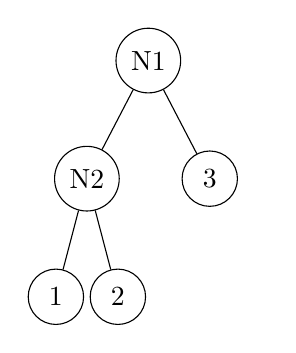
\begin{tikzpicture}
    \Tree
    [.N1  
        [.N2
            \edge[]; {1}
            \edge[]; {2}
        ]
        [.3 
            \edge[blank]; \node[blank]{};
            \edge[blank]; \node[blank]{};
        ]
    ]
\end{tikzpicture}\newline
and as predicate the lambda $\lambda x.x > 1$. The filter function should produce the tree:\newline
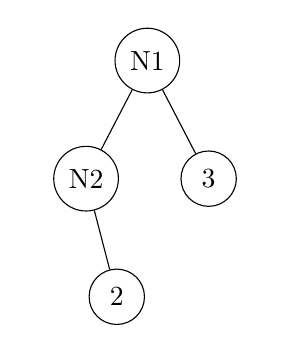
\begin{tikzpicture}
    \Tree
    [.N1  
        [.N2
            \edge[blank]; \node[blank]{};
            \edge[]; {2}
        ]
        [.3 
            \edge[blank]; \node[blank]{};
            \edge[blank]; \node[blank]{};
        ]
    ]
\end{tikzpicture}\newline
We defined our tree type as follows:
\begin{lstlisting}[style = FSharpStyle]
    type 'a tree  = Leaf of 'a | Node of 'a tree * 'a tree
\end{lstlisting}
As you can see, it doesn't support trees with only one child, but we can only represent trees with two children. So, in order to implement the filter function, we need to change the definition and make it more flexible. We can do it in different ways:
\begin{lstlisting}[style = FSharpStyle]
    type 'a tree =
        | Leaf of 'a
        | Node of 'a tree * 'a tree
        | OneChild of 'a tree
\end{lstlisting}
The code above defines a union type with an additional data-constructor which represent a node with only one child. However, we wouldn't be able to distinguish between left-child and right-child. So, in order to obtain this distinction, we can specify two equivalent data-constructors with different names.
\begin{lstlisting}[style = FSharpStyle]
    type 'a tree =
        | Leaf of 'a
        | Node of 'a tree * 'a tree
        | LeftChild of 'a tree
        | RightChild of 'a tree
\end{lstlisting}
We can get the same result by using \textbf{option} type and defining just 2 data-constructor:
\begin{lstlisting}[style = FSharpStyle]
    type 'a tree  = 
        |Leaf of 'a option
        |Node of 'a tree * 'a tree
\end{lstlisting}
In this case, leaves may or may not contain an information. We express the concept of having only one child by defining binary trees that can have \textbf{empty} leaves.\newline\newline
Let's define the filter function according to this tree type definition:
\begin{lstlisting}[style = FSharpStyle]
    let rec filter_tree p t =
        match t with
        | Leaf (Some x) -> if p x then Leaf (Some x) else Leaf None
        | Leaf None -> Leaf None
        | Node (l, r) -> Node (filter_tree p l, filter_tree p r)

    let N = Node
    let L x = Leaf (Some x)
    let tree = N(N(L 1, L 2), L 3)
    let t1 = filter_tree (fun x -> x > 1) tree

    // val filter_tree : p:('a -> bool) -> t:'a tree -> 'a tree
    // val t1 : int tree = Node (Node (Leaf None, Leaf (Some 2)), Leaf (Some 3))
\end{lstlisting}
As you can see, t1 is a tree with an empty leaf that represents the tree presented before.
\subsection{Map and sum functions}
Let's change the map\_tree and sum\_tree functions according to the new tree type definition:
\begin{lstlisting}[style = FSharpStyle]
    let rec map_tree f =
        let R t = map_tree f t
        in fun t ->
            match t with
            | Leaf None -> Leaf None
            | Leaf (Some x) -> Leaf (Some(f x))
            | Node (l, r) -> Node (R l, R r)

    let t2 = map_tree (fun x -> x>1) tree
    
    (*val map_tree : f:('a -> 'b) -> ('a tree -> 'b tree)
      val t2 : bool tree = 
        Node (Node (Leaf (Some false), Leaf (Some true)), Leaf (Some true))*)
\end{lstlisting}

\begin{lstlisting}[style = FSharpStyle]
    let rec sum_tree (+) zero t =
        match t with
        | Leaf (Some x) -> x
        | Leaf None -> zero
        | Node (l, r) -> (sum_tree (+) zero l) + (sum_tree (+) zero r)
\end{lstlisting}
Note that we added the base case of sum (parameter 'zero') that is returned when the function reaches an empty leaf.
\subsection{Union types and pattern-matching in Java}
In order to implement the same thing in an object oriented programming language such as Java, we have to simulate union types using objects and inheritance.\newline\newline
Let's define the map\_tree function in Java:
\begin{lstlisting}[style = JavaStyle]
    public abstract class Tree<T> {
        public abstract <S> Tree<S> map(Function<T, S> f);
    }
    public class Leaf<T> extends Tree<T> {
        @Nullable
        private T data;
        public Leaf(T data) {
            this.data = data;
        }
        @Override
        public <S> Tree<S> map(Function<T, S> f) {
            return new Leaf<S>(data != null ? f.apply(this.data) : null);
        }
    }
    public class Node<T> extends Tree<T> {
        private Tree<T> left, right;
        public Node(Tree<T> l, Tree<T> r) {
            this.leaf = l;
            this.right = r;
        }
        @Override
        public <S> Tree<S> map(Function<T, S> f) {
            return new Node<S>(left.map(f), right.map(f));
        }
    }
\end{lstlisting}
Basically, the map\_tree higher-order function becomes a method of the super-class \textit{tree}, and we simulate pattern-matching by splitting each implementation of map\_tree in the sub-classes (\textit{Leaf} and \textit{Node}). This solution is called \textbf{visitor pattern}. As you can see, the Java code is more complex and long than the F\# code.
\section{Fold function for trees}
\begin{lstlisting}[style = FSharpStyle]
    let rec fold_tree f z t =
        match t with
        | Leaf (Some x) -> f z x
        | Leaf None -> z
        | Node (l,r) ->
            let z' = fold_tree f z l
            fold_tree f z' r
\end{lstlisting}
\begin{itemize}
    \item When the function reaches a leaf that contains an information, it computes the new state of the accumulator by applying the function f. If the leaf is empty, it just returns the accumulator.
    \item When the function reaches a node, it forwards the accumulator computed on the left sub-tree to the right sub-tree.
\end{itemize}
Note that for lists there are two implementations of the fold function: fold-left and fold-right.
\begin{itemize}
    \item \textbf{fold-left: }First computes the accumulator and then performs the recursion step.
    \item \textbf{fold-right: }Recursively goes to the end of the list and \textit{updates} the accumulator in ascension.
\end{itemize}
Since our trees definition doesn't support information in the nodes, we can't distinguish between fold-left and fold-right.

\chapter{Lec 14 - Dealing with Uncertainty}
\section{Uncertainty}
Agents may need to handle \textbf{uncertainty}, whether due to partial observability, nondeterminism, or a combination of the two. Suppose, for example, that an automated taxi has the goal of delivering a passenger to the airport on time. The agent forms a plan, $A_{90}$, that involves leaving home 90
minutes before the flight departs and driving at a reasonable speed. Even though the airport is only about 5 miles away, a logical taxi agent will not be able to conclude with certainty that “Plan $A_{90}$ will get us to the airport in time.” Instead, it reaches the weaker conclusion “Plan $A_{90}$ will get us to the airport in time, as long as the car doesn’t break down or run out of gas, and I don’t get into an accident, and there are no accidents on the bridge, and the plane doesn’t leave early, and no meteorite hits the car, and ... .”  None of these conditions can be deduced for sure, so the plan’s success cannot be inferred. Other plans, such as $A_{180}$, might increase the agent’s belief that it will get to the airport on
time, but also increase the likelihood of a long wait. \textit{The right thing to do, the rational decision, therefore depends on both the relative importance of various goals and the likelihood that, and degree to which, they will be achieved.}
\newline\newline
A logical agent believes each sentence to be true or false or has no opinion, whereas a probabilistic agent may have a numerical degree of belief between 0 (for sentences that are certainly false) and 1 (certainly true). \textbf{Probability} provides a way of summarizing the uncertainty that comes from our
\begin{itemize}
    \item \textbf{laziness:}  failure to enumerate exceptions, qualifications, etc.
    \item \textbf{ignorance}: lack of relevant facts, initial conditions, etc.
\end{itemize}
Probabilities relate propositions to one’s own state of knowledge, e.g. $P(A_{25}|\,\, \text{no reported accidents}) = 0.06$. These are not claims of some probabilistic tendency in the current situation, but might be learned from past experience of similar situations. Probabilities of propositions change with new evidence: 
\[P(A_{25}|\,\, \text{no reported accidents, 5 a.m.}) = 0.15\]
Consider again the $A_{90}$ plan for getting to the airport. Suppose it gives us a 97\% chance of catching our flight. Does this mean it is a rational choice? Not necessarily: there might be other plans, such as $A_{180}$, with higher probabilities.  If it is vital not to miss the flight, then it is worth risking the longer wait at the airport. What about $A_{1440}$, a plan that involves
leaving home 24 hours in advance? In most circumstances, this is not a good choice, because although it almost guarantees getting there on time, it involves an intolerable wait.\\\\
To make such choices, an agent must first have \textbf{preferences} between the different possible outcomes of the various plans. We use \textbf{utility theory} to represent and reason with preferences.  Utility theory says that every state has a degree of usefulness, or utility, to an agent and that the agent will prefer states with higher utility. Preferences, as expressed by utilities, are combined with probabilities in the general theory of rational decisions called \textbf{decision theory}:
\[\textit{Decision theory} = \textit{Probability theory} + \textit{Utility theory}\]

\section{Probability notation}
For our agent to represent and use probabilistic information, we need a formal language.
\begin{itemize}
    \item Probabilities such as $P(Cavity = true)=0.1$ and $P(Weather = sunny)=0.72$ are called \textbf{prior} or \textbf{unconditional} probabilities. They refer to degrees of belief in propositions in the absence of any other information.

    \item Most of the time, we have some information, usually called \textbf{evidence}, that has already been revealed. In this case we have the \textbf{conditional} or \textbf{posterior} probability. For example, $P(cavity|toothache)=0.6$. This assertion does \textbf{not} mean “Whenever toothache is true, conclude that cavity is true with probability 0.6”. Rather it means “Whenever toothache is true and we have no further information, conclude that cavity is true with probability 0.6.”  The extra condition is important; for example, if we had the further information that the dentist found no cavities, we definitely would not want to conclude that cavity is true with probability 0.6; instead we need to use $P(cavity|toothache \land \neg cavity)=0.$ Note also that new evidence may be irrelevant, allowing simplification, e.g., $P(cavity|toothache, InterWin) = P(cavity|toothache)=0.6$.\\\\
    Mathematically speaking, conditional probabilities are defined in terms of unconditional probabilities as follows: for any events $a$ and $b$, we have
    \[P(a | b) = \frac{P(a \land b)}{P(b)}\]
    The definition of conditional probability  can be written in a different form called the \textbf{product rule}:
    \[P(a \land b) = P(a|b)P(b)\]
    
    
    
    \item Variables in probability theory are called \textbf{random variables} and their names begin with an uppercase letter. Every random variable has a \textbf{domain}, the set of possible values it can take on. A \textbf{Probability distribution} gives values for all possible assignments to a random variable. E.g., if $Weather$ can take values in \\$<sunny,rain,cloudy,snow>$, then
    \[\textbf{P}(Weather) = <0.72, 0.1, 0.08, 0.1>\]
     Normalized, i.e., sums to 1. For continuous variables, it is not possible to write out the entire distribution as a vector, because there are infinitely many values. Instead, we can define the probability that a random variable takes on some value $x$ as a parameterized function of $x$. We call this a \textbf{probability density function}.

     \item In addition to distributions on single variables, we need notation for distributions on multiple variables. The \textbf{Joint probability distribution} for a set of random variables gives the probabilities of all combinations of the values of those random variables (i.e., every sample point). For example, $\textbf{P}(Weather, Cavity)$ is a $4 \times 2$ table of probabilities:
     \begin{center}
         \includegraphics[]{images/joint-prob.png}
     \end{center}
     Every question about a domain can be answered by the joint distribution because every event is a sum of sample points.\\\\
     Any joint probability distribution over many random variables may be decomposed into conditional distributions.
     \begin{center}
         \includegraphics[]{images/chain-rule.png}
     \end{center}
     This observation is known as the \textbf{chain rule} of probability.
\end{itemize}

\section{Inference by enumeration}
Inference by enumeration means doing inference using only full joint distributions. \textbf{Probabilistic inference} is the computation of posterior probabilities for query propositions given observed evidence.\\\\
We begin with a simple example: a domain consisting of just the three Boolean variables $Toothache$, $Cavity$, and $Catch$ (the dentist’s nasty steel probe catches in my tooth). The full joint distribution is a $2 \times 2 \times 2$ table.
\begin{center}
    \includegraphics[]{images/dentist-table.png}
\end{center}
The probability associated with a proposition is defined to be the sum of the probabilities of the atomic events in which it holds: For any proposition $\phi$
\[P(\phi) = \sum_{w \in \phi}P(w)\]
For example, when rolling fair dice, we have $P(Total = 11) = P((5, 6)) + P((6, 5)) = 1/36 + 1/36 = 1/18$. \\\\
Then, we can calculate the probability $P(cavity \lor toothache)$ as follows:
\[P(cavity \lor toothache) = 0.108 + 0.012 + 0.072 + 0.008 + 0.016 + 0.064 = 0.28\]
We  simply identify those events in which the proposition is true and add up their probabilities.
\begin{center}
    \includegraphics[]{images/dentist-table-2.png}
\end{center}
One particularly common task is to extract the distribution over some subset of variables or a single variable. For example, adding the entries in the first row gives the unconditional or \textbf{marginal probability} of cavity:
\[P(cavity) = 0.108 + 0.012 + 0.072 + 0.008 = 0.2\]
This process is called \textbf{marginalization}, or \textbf{summing out}, because we sum up the probabilities for each possible value of the other variables. We can write the following general marginalization rule for any sets of variables $\textbf{Y}$ and $\textbf{Z}$:
\[\textbf{P}(\textbf{Y}) = \sum_{\textbf{z} \in \textbf{Z}}\textbf{P}(\textbf{Y}, \textbf{z})\]
where $\sum_{\textbf{z} \in \textbf{Z}}$ means to sum over all the possible combinations of values of the set of variables $\textbf{Z}$.
\[\textbf{P}(Cavity) = \sum_{\textbf{z} \in \{Catch, Toothache\}} \textbf{P}(Cavity, \textbf{z})\]
We can also compute conditional probabilities, for example:
\[
\begin{split}
    P(cavity | toothache) & = \frac{P(cavity \land toothache)}{P(toothache)}\\
    & = \frac{0.108 + 0.012}{0.108 + 0.012 + 0.016 + 0.064}\\
    & = 0.6
\end{split}
\]
Just to check, we can also compute the probability that there is no cavity, given a toothache:
\[
\begin{split}
    P(\neg cavity | toothache) & = \frac{P(\neg cavity \land toothache)}{P(toothache)}\\
    & = \frac{0.016 + 0.064}{0.108 + 0.012 + 0.016 + 0.064}\\
    & = 0.4
\end{split}
\]
The two values sum to 1.0, as they should. Notice that in these two calculations the term $1/P(toothache )$ remains constant, no matter which value of $Cavity$ we calculate. In fact, it can be viewed as a normalization constant for the distribution $\textbf{P}(Cavity |toothache)$, ensuring that it adds up to 1. With this notation, we can write the two preceding equations in one:
\begin{center}
    \includegraphics[]{images/prob-inference-rule.png}
\end{center}
Where $\alpha$ is the normalization constant. In other words, we can calculate $\textbf{P}(Cavity |toothache)$ even if we don’t know the value of $P(toothache)$. We temporarily forget about the factor $1/P(toothache )$ and add up the values for $cavity$ and $\neg cavity$, getting 0.12 and 0.08. Those are the correct relative proportions, but
they don’t sum to 1, so we normalize them by dividing each one by 0.12 + 0.08, getting the true probabilities of 0.6 and 0.4.\\\\
From the example, we can extract a general inference procedure. We begin with the case in which the query involves a single variable, $X$ (Cavity in the example).  Let $\textbf{E}$ be the list of evidence variables (just $Toothache$ in the example), let $\textbf{e}$ be the list of observed values for them,  and let $\textbf{Y}$ be the remaining unobserved (hidden) variables (just $Catch$ in the example). The query is $\textbf{P}(X | \textbf{e})$ and can be evaluated as:
\[\textbf{P}(X | \textbf{e}) = \alpha \textbf{P}(X, \textbf{e}) = \alpha \sum_{\textbf{y}}\textbf{P}(X, \textbf{e}, \textbf{y})\]
where the summation is over all possible $\textbf{y}$s (i.e., all possible combinations of values of the unobserved variables $\textbf{Y}$).\\\\
Given the full joint distribution to work with, this inference procedure can answer probabilistic
queries for discrete variables. It does not scale well, however: for a domain described by $n$ Boolean variables, it requires an input table of size $O(2^n)$ and takes $O(2^n)$ time to process the table.

\section{Independence}
Two variables $X$ and $Y$ are \textbf{independent} iff
\[\textbf{P}(X | Y ) = \textbf{P}(X)\,\, \text{or} \,\,\textbf{P}(Y | X) = \textbf{P}(Y)\,\, \text{or}\,\, \textbf{P}(X, Y ) = \textbf{P}(X)\textbf{P}(Y )\]
Let us expand the full joint distribution seen before by adding a fourth variable, $Weather$. The full joint distribution then becomes $\textbf{P}(Toothache, Catch, Cavity,Weather )$, which has $2 \times 2 \times 2 \times 4 = 32$ entries. We may ask how these variables are related, for example, how are $P(toothache, catch, cavity, cloudy)$
and $P(toothache, catch, cavity)$ related? We can use the product rule:
\[P(toothache, catch, cavity, cloudy)
= P(cloudy |toothache, catch, cavity)P(toothache, catch, cavity)\]
Now, it seems safe to say that the weather does not influence the dental variables. Therefore, the following assertion seems reasonable:
\[P(cloudy |toothache, catch, cavity) = P(cloudy)\]
From this, we can deduce:
\[P(toothache, catch, cavity, cloudy) = P(cloudy)P(toothache, catch, cavity)\]
A similar equation exists for every entry in $\textbf{P}(Toothache, Catch, Cavity,Weather)$. In fact, we can write the general equation:
\[\textbf{P}(Toothache, Catch, Cavity, Weather ) = \textbf{P}(Toothache, Catch, Cavity)\textbf{P}(Weather ) .\]
Therefore, the weather is independent of one’s dental problems.\\\\
If the complete set of variables can be divided into independent subsets, then the full joint distribution can be \textbf{factored} into separate joint distributions on those subsets. In a more practical vein, the independence of
dentistry and meteorology is a good thing, because otherwise the practice of dentistry might require intimate knowledge of meteorology, and vice versa. When they are available, then, independence assertions can help in reducing the size of
the domain representation and the complexity of the inference problem. Unfortunately, clean separation of entire sets of variables by independence is quite rare.


\chapter{Lec 15-16 Part I - Type inference in F\#}

\section{Simple type inference algorithm}
The type inference algorithm automatically understands the type of an expression in a formal language. Let's consider the following F\# functions with their respective types:
\begin{lstlisting}[style=FSharpStyle]
    let f a b c = if a then b c else a
    //val f : a:bool -> b:('a -> bool) -> c:'a -> bool
    
    let g x y z = (x, y, z)
    //val g : x:'a -> y:'b -> z:'c -> 'a * 'b * 'c

    let h x y z = z y x
    //val h : x:'a -> y:'b -> z:('b -> 'a -> 'c) -> 'c
\end{lstlisting}
A simple type inference high-level algorithm could be the following:
\begin{enumerate}
    \item Bind unknown types to the parameters ('a, 'b, 'c, ...). We will call these unknown types \textbf{type variables}.
    \item \textbf{Substitute} each type variable with a concrete type (if possible) according to what is written in the body of the function. Once a concrete type (int, float, bool, ...) is fixed, it doesn't change anymore. If we need to substitute more that one concrete type it means there is an error in the function.
\end{enumerate}
For example, if we change the definition of f as follows:
\begin{lstlisting}[style=FSharpStyle]
    let f a b c = if a then b c else a+1
\end{lstlisting}
it produces an error because \textit{a} was inferred as bool but is used as an int in the \textit{else} branch of the \textit{if-then-else} statement.
\begin{lstlisting}[style=FSharpStyle]
    let f a b c = if a+1 > 3 then b c else a
\end{lstlisting}
Since the \textit{if-then-else} statement must return the same type in both the branches, the type of the new definition of f is:
\begin{lstlisting}[style=FSharpStyle]
    int -> ('a -> int) -> 'a -> int
\end{lstlisting}
\begin{itemize}
    \item \textit{a} has type int
    \item Also the function \textit{b} produces an int
\end{itemize}
In the body of the function g there are no \textbf{constraints} that permit the type inference to substitute any concrete type, so it will remain a polymorphic function with respect to all the parameters.\newline\newline
Let's insert a constraint in the body of the function g.
\begin{lstlisting}[style=FSharpStyle]
    let g x y z = (x-1, y, z)
\end{lstlisting}
With this change, the compiler understands that \textit{x} must be an integer (due to the constraint x-1), while y and z remain unknown (polymorphic). Polymorphism arises from not knowing any constraint on a type. \newline\newline
Now we can define a more detailed pipeline of the type inference algorithm:
\begin{enumerate}
    \item Bind unknown types to parameters (type variables)
    \item Create a list of constraints according to the body of the function
    \item Check the list of constraints:
           \begin{enumerate}
               \item Eliminate trivial constraints
               \item If two or more constraints for the same type variable are found, produce an error
           \end{enumerate} 
    \item Substitute to each type variable a concrete type, according to the constraints list, to find the final type.    
\end{enumerate}
Let's make an example:
\begin{lstlisting}[style=FSharpStyle]
    let j x = if x then x else x
\end{lstlisting}
\begin{enumerate}
    \item We start by binding unknown types:
    \begin{lstlisting}[style=FSharpStyle]
        j: 'a -> 'b
    \end{lstlisting}
    \item The \textit{if-then-else} statement requires two constraints:
        \begin{itemize}
            \item The guard of the \textit{if} must be a bool
            \item The two branches must produce the same type
        \end{itemize}
    So the list of constraints becomes:
    \begin{lstlisting}[style=FSharpStyle]
        'a -> bool
        'a -> 'a
        'b -> 'a
    \end{lstlisting}
    By eliminating trivial constraints the list becomes:
    \begin{lstlisting}[style=FSharpStyle]
        'a -> bool
        'b -> 'a
    \end{lstlisting}
    Then, we simplify the constraints list:
    \begin{lstlisting}[style=FSharpStyle]
        'a -> bool
        'b -> bool
    \end{lstlisting}
    \item Since there are not multiple constraints for the same type variable, we can perform the substitution. The type of j becomes:
    \begin{lstlisting}[style=FSharpStyle]
        j: bool -> bool
    \end{lstlisting}
    The substitution can be seen as a function from type variables to types:
    \[ \Theta: \alpha \rightarrow \tau\]
\end{enumerate}
Note that if we had written the following expression:
\begin{lstlisting}[style=FSharpStyle]
    let j x = if x then x else 2
\end{lstlisting}
the constraints list would have been:
\begin{lstlisting}
    'a -> bool
    'a -> int
    'b -> int
\end{lstlisting}
So, the type inference algorithm would have produced an error since there are multiple constraints for the type variable 'a.


\chapter{Lec 15-16 Part II - Type checking rule}

\section{Inference logic rule}
\[
    \infer{\Gamma \vdash \lambda x.e : \tau_{1} \rightarrow \tau_{2}}{\Gamma, (x:\tau_{1}) \vdash e:\tau_{2}}\]
The formula above, in the world of logic, is called \textbf{inference logic rule}. Basically, it is an implication from "\textit{up}" to "\textit{down}". It means that the formula above the horizontal line implies the formula below.\newline\newline
In order to understand this rule, we need to define its terms.
\subsection{Expressions}
\label{expr}
$e$ is an \textbf{expression} defined through a \textbf{BNF} grammar:
\begin{grammar}
    <e> ::= <x>
    \alt <λx.e> 
    \alt <e e>
    \alt <Let x = e in e>
\end{grammar}
An expression $e$ can either be:
\begin{itemize}
    \item A variable name
    \item A lambda
    \item An application
    \item A let binding
\end{itemize}
Let's consider the following expression in F\#:
\begin{lstlisting}[style=FSharpStyle]
    let m = (1+2+3) 4
\end{lstlisting}
The right part of the let binding is correct from the point of view of the syntax (it's an application), but is wrong from the point of view of types. So, a compiler can be seen as a pipeline:
\begin{enumerate}
    \item First checks the syntax
    \item Then understands types (type inference)
\end{enumerate}
    
\subsection{Types}
A type $\tau$ is defined as a syntactic entity through a BNF grammar:
\begin{grammar}
    <τ> ::= <c>
    \alt <τ ⟶ τ >
    \alt α
\end{grammar}
Where $c$ is a constant type name (e.g. int, float, bool, ...) and $\alpha$ is a \textbf{generic} type variable.

\subsection{The environment $\Gamma$}
$\Gamma$ is the environment (scope) and is defined as follows:
\begin{grammar}
    <Γ> ::= Ø
    \alt <Γ,(x : τ) >
\end{grammar}
Let's consider the following F\# code:
\begin{lstlisting}[style=FSharpStyle]
    let f a b c = if a then b c else a

    let myfun x y=
        let f z = f x y x
        f 3
\end{lstlisting}
Note that when we bind \textit{f} inside \textit{myfun}, since it is not specified the \textbf{rec} keyword, we are referring to the definition of \textit{f} written above \textit{myfun}. So, in order to analyze the type of the nested function \textit{f} defined inside \textit{myfun}, the compiler must have memorized the type of the function \textit{f} defined above \textit{myfun}. In F\# the let binding adds an entry to the scope, but how can we represent this information ? \newline\newline
The simplest way for representing the scope is a sequence of pairs, where each pair is composed by an identifier and its type. $\Gamma$ can be seen as a function from the set of identifiers $X$ to types:
\[\Gamma: X \rightarrow \tau\]
\subsection{Understanding the formula}
Let's go back to the logic rule mentioned before:
\[
    \infer{\Gamma \vdash \lambda x.e : \tau_{1} \rightarrow \tau_{2}}{\Gamma, (x:\tau_{1}) \vdash e:\tau_{2}}\]
\begin{itemize}
    \item $\vdash$ means "\textit{deduce}"
    \item : means "\textit{has type}"
\end{itemize}
so, a literal translation of $\Gamma \vdash e : \tau$ would be: "\textit{In a scope $\Gamma$, we deduce that the expression $e$ has type $\tau$}".\newline\newline
The meaning of the whole formula is the following: Given a lambda $\lambda x.e$ in an environment $\Gamma$, if we extend the scope $\Gamma$ by binding to the parameter $x$ the type $\tau_{1}$ and we deduce that the body $e$ has type $\tau_{2}$, then the lambda must have type $\tau_{1} \rightarrow \tau_{2}$.  Basically, it says that the domain of the lambda is the type of the parameter and the codomain is the type of the body.\newline\newline
This is a \textbf{type checking} rule because it says what must be true for an expression in order to be valid from the point of view of types, but it doesn't show how to infer types. Type inference shows how to automatically understands types, rather than just assuming them.\newline\newline
Let's make an example in F\#:
\begin{lstlisting}[style=FSharpStyle]
    let r  = fun x -> x 23
\end{lstlisting}
The right part of the let binding is a lambda that has an application as body. The type inference understands that:
\begin{itemize}
    \item the parameter $x$ has type int $\rightarrow$ 'a
    \item the expression $e$, that is an application, has type 'a
\end{itemize}
Then, by applying the type checking rule, the whole lambda must have type (int $\rightarrow$ 'a) $\rightarrow$ 'a\newline\newline
It is useful to express the type checking algorithm through a series of logical implications. This is because we want to describe the algorithm in such a way that we can derive some mathematical properties. The most important property that we can derive from this definition is \textbf{soundness}.\newline\newline
Soundness means that given a program, if the types are correct then the program works (in the sense that run without crashing). Note that, in functional languages, every program is an expression made of multiple let bindings.
\subsection{Type checking rule for the other expression terms}
We defined the type-checking rule only for the lambda-term of expressions. Let's write the same rule with respect to application, variable name and let binding terms (according to the definition of expression we gave in section \ref{expr}). 
\begin{itemize}
    \item \textbf{Variable name:} 
    \[ \infer{\Gamma \vdash x : \tau}{ \begin{gathered} x \in domain(\Gamma)\\ \Gamma(x) = \tau \end{gathered}} \]
    A variable $x$ has type $\tau$ in the scope $\Gamma$ if it is defined in the scope and if $\Gamma$ applied to $x$ produces $\tau$ ($\Gamma$ is a function as we said previously).
    \item \textbf{Application:} 
    \[ \infer{\Gamma \vdash e_{1} \, e_{2} : \tau_{2}}{\begin{gathered} \Gamma \vdash e_{1} : \tau_{1} \rightarrow \tau_{2} \\ \Gamma \vdash e_{2} : \tau{1} \end{gathered}}\]

    \item \textbf{Let binding:}
    \[ \infer{\Gamma \vdash let \, x = e_{1} \, in \, e_{2} : \tau_{2}}{\begin{gathered}
        \Gamma \vdash e_{1} : \tau_{1}\\
        \Gamma, (x:\tau_{1}) \vdash e_{2}:\tau_{2}
    \end{gathered}}\]
    Let's make an example in F\#:
    \begin{lstlisting}[style=FSharpStyle]
        let a=3 in let b = true in a
    \end{lstlisting}
    In this example $e_{1} = 3$ and $e_{2} =$ \textit{let b = true in a }. The rule that type checks the binding \textit{let a = 3} is $\Gamma \vdash e_{1}:\tau_{1}$. In our example $\tau_{1}=int \rightarrow e_{1}:int$. Then, we bind \textit{(a:int)} and we add this information to the original scope. By recursively repeating the type-checking for $e_{2}$ in the extended scope, we'll eventually have the environment $\Gamma$ composed by: $\{(a:int), (b:int)\}$ and the variable \textit{a}
    will be type-checked following the rule mentioned before. 
\end{itemize}


\chapter{Lec 16 - Bayesian Learning II}

\section{Naive Bayes Classifier}
One of the simplest and most popular techniques based on Bayesian learning is the \textbf{Naive Bayes classifier}. It is an effective method when we have large data-sets and when the attributes describing the instances are conditionally independent given the classification.\newline\newline
Given a target function $f: X \rightarrow V$, with instances $x$ described by a set of attributes $\langle a_{1}, a_{2},...,a_{n}\rangle$, the most probable classification of a new instance $f(x)$ is:
\[v_{MAP} = argmax_{v_{j} \in V}P(v_{j} | a_{1}, a_{2},...,a_{n})\]
We want to maximize the probability to have class $v_{j}$ given the values of the instance attributes. By resorting to the Bayes formula, it follows that:
\[= argmax_{v_{j} \in V} \frac{P(a_{1}, a_{2},...,a_{n} | v_{j})P(v_{j})}{P(a_{1}, a_{2},...,a_{n})}\]
Note that $P(a_{1}, a_{2},...,a_{n})$ does not depend on $v_{j}$, so we can consider it as a constant and remove it from the formula:
\[= argmax_{v_{j} \in V} P(a_{1}, a_{2},...,a_{n} | v_{j})P(v_{j})\]
\begin{itemize}
    \item Compute $P(v_{j})$ is easy. We can compute the ratio between the occurrences of instances of class $v_{j}$ and the number of instances in the training set.

    \item Estimate $P(a_{1}, a_{2},...,a_{n} | v_{j})$ is \textbf{impossible}. This is because, since we should compute a probability for each combination of $a_{1}, a_{2},...,a_{n}$, which is computationally unfeasible. Furthermore, we need to see every  instance in the instance space many times in order to obtain reliable estimates. Hence, we would have a very, very large set of training data.
\end{itemize}
So, in order to overcome this problem, the Naive Bayes method makes an assumption:
\[P(a_{1}, a_{2},...,a_{n} | v_{j}) = \prod_{i}P(a_{i}|v_{j})\]
which means that the attributes describing an instance are independent each other.\newline\newline
Finally, the most probable class according to the Naive Bayes classifier is given by the following formula:
\[v_{NB} = argmax_{v_{j} \in V}P(v_{j})\prod_{i}P(a_{i}|v_{j})\]
One interesting difference between the naive Bayes learning method and other learning methods is that there is no explicit search through the space of possible hypotheses (in this case,  the  space of possible hypotheses is the space of possible values that can be assigned to the various $P(v_j)$ and $P(a_i|v_j)$ terms). Instead, the hypothesis is formed without searching, simply by counting the frequency of various data combinations within the training examples.

\subsection{Naive Bayes algorithm}
Given a training set $Tr$:
\begin{enumerate}
    \item For each target value $v_{j}$
    \begin{enumerate}
        \item $\hat{P}(v_{j}) \leftarrow$ estimate $P(v_{j})$ on $Tr$
        \item $\forall a_{i}$: $\hat{P}(a_{i} | v_{j}) \leftarrow$ estimate $P(a_{i} | v_{j})$ on $Tr$ (using the ratio method as done for $P(v_{j})$)
    \end{enumerate}
    \item return $\hat{P}(v_{j})$, $\hat{P}(a_{i} | v_{j})$ $\forall i,j$
\end{enumerate}
The \textbf{classification} of a new instance $x$ works as follows:
\begin{enumerate}
    \item $v_{NB} = argmax_{v_{j} \in V}\hat{P}(v_{j})\prod_{i}\hat{P}(a_{i}(x) | v_{j})$
    \item return $v_{NB}$
\end{enumerate}
where $a_{i}(x)$ is the value of the $i$-th attribute of the instance $x$.

\subsection{Naive Bayes: additional considerations}
The assumption of conditional independence is often violated, that is:
\[P(a_{1}, a_{2},...,a_{n}|v_{j}) \neq \prod_{i}P(a_{i}|v_{j})\]
Despite this, the Naive Bayes algorithm still works. This is because it is not necessary to correctly estimate the posterior probability $\hat{P}(v_{j}|x)$. It is sufficient that the order of those probability is \textit{correct}.\newline\newline
Note that if no training examples with target value $v_{j}$ has the attribute value $a_{i}$ equal to $k$, it follows that:
\[\hat{P}(a_{i} = k | v_{j}) = 0, \,\, and \,\, \hat{P}(v_{j})\prod_{i}\hat{P}(a_{i}|v_{j}) = 0\]
This can compromise the classification of the Naive Bayes method. A typical solution is the Bayesian \textit{m-estimate} for $\hat{P}(a_{i} | v_{j})$:
\[\hat{P}(a_{i} = k | v_{j}) \leftarrow \frac{n_{c} + mp_{k}}{n + m}\]
where:
\begin{itemize}
    \item $n$ is the number of training examples where $v = v_{j}$
    \item $n_{c}$ is the number of training examples where $v = v_{j}$ and $a = a_{i}$
    \item $p$ is the prior estimate of $\hat{P}(a_{i} | v_{j})$.
    \item $m$ is a constant which determines how heavily to weight $p$
\end{itemize}
Applications for Naive Bayes classifier are:
\begin{itemize}
    \item Diagnosis
    \item Classification of textual documents
\end{itemize}
In the context of text classification, it can be used to:
\begin{itemize}
    \item learn which documents are of interest
    \item learn to classify web pages by topic
    \item spam / no spam
    \item ...
\end{itemize}

\section{Learning to classify a text}
Given a document ($doc$), we want to classify it as interesting or not interesting for a particular user: $doc \rightarrow \{+, -\}$. We can represent a document by a vector of words where each word position in the document is an attribute:
\[doc = \{a_{1} = w_{1}, a_{2} = w_{2},..., a_{n} = w_{n}\}\]
We need to estimate the following probabilities:
\[P(+), \,\, P(-), \,\, P(doc | +), \,\, P(doc | -)\]
In this case, in addition to the assumption of conditional independence made before, we have to make another one:
\[P(a_{i} = w_{k} | v_{j}) = P(a_{m} = w_{k} | v_{j}), \,\, \forall i, j, k, m\]
where $P(a_{i} = w_{k} | v_{j})$ is the probability that the word in position $i$ is $w_{k}$, given $v_{j}$. Basically, we assume that the probability for each word to appear in any position is the same.\newline\newline
Therefore, we need to estimate \textit{only} the $P(v_{j}) \,\, \forall j$ and $P(w_{k} | v_{j}) \,\, \forall k, j$.\newline\newline
We can use a $m$-estimate with uniform priors and $m$ equal to the size of the vocabulary:
\[\hat{P}(w_{k} | v_{j}) = \frac{n_{k} + 1}{n + |Vocabulary|}\]
where
\begin{itemize}
    \item $n$ is the total number of word positions in all training documents having class $v_{j}$

    \item $n_{k}$ is the number of times the word $w_{k}$ is in these positions

    \item $|Vocabulary|$ is the total number of distinct words found in the training set.
\end{itemize}
\begin{center}
    \includegraphics[]{images/training_naive_bayesian.png}
\end{center}




\end{document}
